%!TEX root =../mapp-challenge-18-game-book.tex
% ^ leave for LaTeXTools build functionality

\phChapterWorksheet{Route to Victory}{Metapuzzle}

You've finally reached the end of your journey, having been honored
by the four \textbf{Dojo Masters} with the opportunity to compete with them
and three other trainers in the \textbf{\mappMobimon{} Tournament}! You've
each been ranked according to your previous battle experience; unfortunately,
that means you'll have to work your way up from the bottom!

\begin{center}
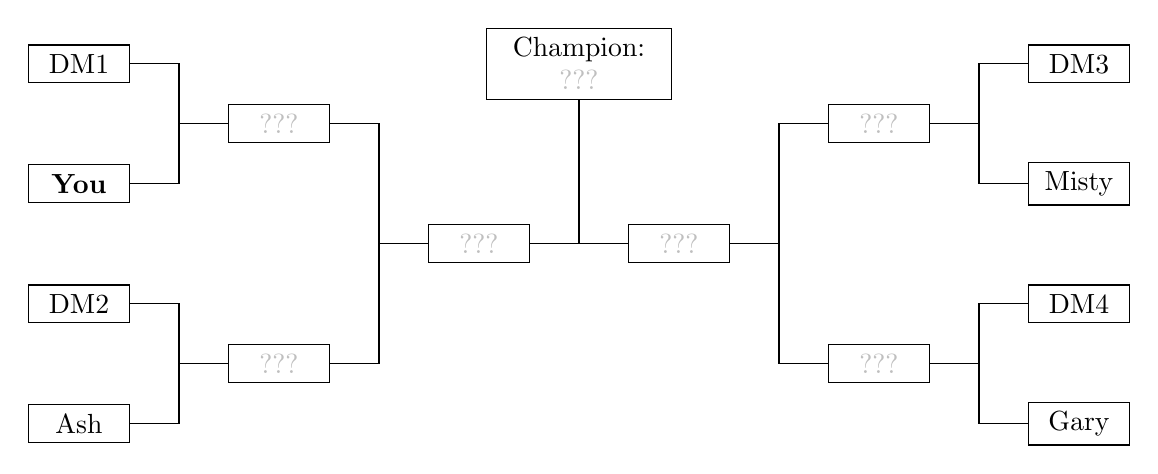
\begin{tikzpicture}[x=0.5in,y=0.3in,every node/.style={rectangle,fill=white,draw,align=center,text width=3em}]
  \draw (0,0) -- (1,0) -- (1,1) -- (3,1) -- (3,3) -- (7,3) --
        (7,1) -- (9,1) -- (9,0) -- (10,0);
  \draw (0,2) -- (1,2) -- (1,1);
  \draw (10,2) -- (9,2) -- (9,1);
  \draw (0,6) -- (1,6) -- (1,5) -- (3,5) -- (3,3);
  \draw (10,6) -- (9,6) -- (9,5) -- (7,5) -- (7,3);
  \draw (0,4) -- (1,4) -- (1,5);
  \draw (10,4) -- (9,4) -- (9,5);
  \draw (5,6) -- (5,3);
  \node at (0,6) {DM1};
  \node at (0,4) {\textbf{You}};
  \node at (0,2) {DM2};
  \node at (0,0) {Ash};
  \node at (2,1) {\textcolor{black!25}{???}};
  \node at (2,5) {\textcolor{black!25}{???}};
  \node at (4,3) {\textcolor{black!25}{???}};
  \node[text width=6em] at (5,6) {Champion: \textcolor{black!25}{???}};
  \node at (6,3) {\textcolor{black!25}{???}};
  \node at (8,1) {\textcolor{black!25}{???}};
  \node at (8,5) {\textcolor{black!25}{???}};
  \node at (10,6) {DM3};
  \node at (10,4) {Misty};
  \node at (10,2) {DM4};
  \node at (10,0) {Gary};
\end{tikzpicture}
\end{center}

\begin{multicols}{2}\small
\begin{itemize}
  \item Dojo Master 1 (Rank 1) will use \underline{\hspace{6em}}.
  \item Dojo Master 2 (Rank 2) will use \underline{\hspace{6em}}.
  \item Dojo Master 3 (Rank 3) will use \underline{\hspace{6em}}.
  \item Dojo Master 4 (Rank 4) will use \underline{\hspace{6em}}.
  \item Gary (Rank 5) will use Glowmage.
  \item Misty (Rank 6) will use Squidiny.
  \item Ash (Rank 7) will use Steinape.
  \item You (Rank 8) will use \underline{\hspace{6em}}.
\end{itemize}
\begin{itemize}
  \item 1st place \mappMobimon{}: \underline{\hspace{10em}}
  \item 2nd place \mappMobimon{}: \underline{\hspace{10em}}
  \item 3rd place \mappMobimon{}: \underline{\hspace{10em}}
  \item 4th place \mappMobimon{}: \underline{\hspace{10em}}
  \item 5th place \mappMobimon{}: \underline{\hspace{10em}}
  \item 6th place \mappMobimon{}: \underline{\hspace{10em}}
  \item 7th place \mappMobimon{}: \underline{\hspace{10em}}
  \item 8th place \mappMobimon{}: \underline{\hspace{10em}}
\end{itemize}
\end{multicols}

Your task is no simple one, so be sure to read over the
\textbf{\mappMobimon{} Battling Overview} to learn the ins and outs
of the tournament.

\begin{itemize}
  \item You should be able to \textbf{figure out which \mappMobimon{}} each of
        the Dojo Masters will use in this tournament
        based upon your previous experiences with them and the provided
        \textbf{\mappMobimon{} List}.
  \item You'll also need to \textbf{choose a \mappMobimon{} for yourself}.
        Luckily, there's exactly one \mappMobimon{} on the provided list that
        can beat every trainer you'll face in the tournament!
  \item Finally, if you \textbf{rank the participating \mappMobimon{}} according
        to the tournament results, you might be able to identify a common
        nickname for the \mappMobimon{} Champion, solving today's final
        puzzle!
\end{itemize}


\phWorksheet{\mappMobimon{} Battling Overview}

The \(PWR\) of a \mappMobimon{} move is based on the
\mappMobimon{}'s \(LV\), but modified by a couple rules.

Each \mappMobimon{} has one or two of these types: Ordinary, Flame, Aqua, Plant,
Magic, Undead, and Lightning. In addition, each \mappMobimon{} move has one
of those types as well. If the type of the move matches one of its user's
types, then the \(PWR\) of that move is multiplied by \(1.5\). Otherwise
the \mappMobimon{} type does not affect the \(PWR\) of the move at all.

Secondly, the type(s) of the opponent \mappMobimon{} also affect the move's
\(PWR\), according to the following chart.
For each of the opponent's types, consider the cell found in the
intersection of that column and the row given by the move type. If the cell
isn't empty, multiply the move's \(PWR\) by that number.

\begin{center}
\begin{tabular}{c||c|c|c|c|c|c|c|}
     &  O  &  F  &  A  &  P  &  M  &  U  &  L  \\\hline\hline
  O  &     &     &     &     & 1/2 &  0  & 1/2 \\\hline
  F  &     & 1/2 & 1/2 &  2  &     &  2  &     \\\hline
  A  &     &  2  & 1/2 & 1/2 &  2  &     &     \\\hline
  P  &     & 1/2 &  2  & 1/2 &     &     &  2  \\\hline
  M  & 1/2 &  2  &     &     &     &     &  2  \\\hline
  U  &  0  &     &     &  2  &  2  &     &     \\\hline
  L  & 1/2 &     &  2  &     &     &  2  &     \\\hline
\end{tabular}
\end{center}

For example, a Flame-type move used against a Plant/Magic-type
\mappMobimon{} is modified by a factor of \(2\), but it
would be modified by \(\frac{1}{4}\) instead if used against a Flame/Aqua-type
\mappMobimon{}. (If the user has the Flame type, then the total modifers would
be \(3\) and \(\frac{3}{8}\), respectively.)

Each \mappMobimon{} knows two different moves, so it's up to the
trainer to decide which move would have greater \(PWR\) against their
opponent. The \mappMobimon{} that uses the move with greater \(PWR\) than
their opponent wins the battle and moves on in the tournament, and the
loser is knocked out.

During a tournament, each trainer must use the same \mappMobimon{} for all
battles, and each \mappMobimon{} cannot be used by more than one trainer.
At the conclusion of the tournament, the trainers and their
\mappMobimon{} are ranked according
to how many battles were won: 1st place for 3 wins, 2nd place for 2 wins,
3rd-4th place for 1 win, and 5th-8th place for no wins. The rankings each
trainer entered the tournament with are used to sort 3rd-4th and 5th-8th
places.

\phWorksheet{\mappMobimon{} List}

\begin{center}
\begin{tabular}{|c|c|c|c|c|p{2in}|}\hline
  Name & Type(s) & \(LV\) & 1st Move & 2nd Move & Mob\'idex Description \\\hline\hline
  %%%%%%%%%%%%%%%%%%%%%%%%%%%%%%%%%%%%%%%%%%%%%%%%%%%%%%%%%%%%%%%%%%%%%%
  Ariafire & Flame & 50 & Flame & Lightning &
    Works well with other firey \mappMobimon{}. \\\hline
  Burnezam & Flame/Magic & 49 & Flame & Magic &
    Known for its caution and level-headedness. \\\hline
  Dawnoduh & Ordinary/Undead & 56 & Ordinary & Flame &
    Your run-of-the-mill zombie. \\\hline
  Emaphant & Ordinary & 52 & Ordinary & Magic &
    Tramples over the competition. \\\hline
  Finfanta & Magic & 54 & Magic & Flame &
    Moody, it creates clouds of strife. \\\hline
  Glowmage & Magic/Lightning & 55 & Magic & Undead &
    A shining example of magical prowess. \\\hline
  Planktin & Aqua/Plant & 51 & Plant & Ordinary &
    Well, it grows on you at least. \\\hline
  Scorchar & Flame/Lightning & 58 & Flame & Undead &
    It can run a marathon in under 38 minutes. \\\hline
  Steinape & Undead/Lightning & 47 & Lightning & Ordinary &
    It's alive with passion for battling. \\\hline
  Squidiny & Aqua & 57 & Aqua & Ordinary &
    A lot of fun to go surfing with. \\\hline
  Thundora & Lightning & 53 & Lightning & Plant &
    The most profecient of its kind. \\\hline
  Zomtreed & Plant/Undead & 43 & Undead & Magic &
    This extreme \mappMobimon{} pushes it to the limit. \\\hline
\end{tabular}
\end{center}


% Include below for aucTeX integration
%%% Local Variables:
%%% mode: latex
%%% TeX-master: "../mapp-challenge-18-game-book"
%%% End:
